%----------------------------------------------------------------------------------------
%	PACKAGES AND OTHER DOCUMENT CONFIGURATIONS
%----------------------------------------------------------------------------------------

\documentclass[11pt,a4paper,twoside]{article}

\usepackage{lipsum} % Package to generate dummy text throughout this template

\usepackage[sc]{mathpazo} % Use the Palatino font
\usepackage[T1]{fontenc} % Use 8-bit encoding that has 256 glyphs
\linespread{1.05} % Line spacing - Palatino needs more space between lines
\usepackage{microtype} % Slightly tweak font spacing for aesthetics

\usepackage[hmarginratio=1:1,top=32mm,columnsep=20pt]{geometry} % Document margins
\usepackage[hang, small,labelfont=bf,up,textfont=it,up]{caption} % Custom captions under/above floats in tables or figures
\usepackage{booktabs} % Horizontal rules in tables
\usepackage{float} % Required for tables and figures in the multi-column environment - they need to be placed in specific locations with the [H] (e.g. \begin{table}[H])
\usepackage{hyperref} % For hyperlinks in the PDF

\usepackage{lettrine} % The lettrine is the first enlarged letter at the beginning of the text
\usepackage{paralist} % Used for the compactitem environment which makes bullet points with less space between them

\usepackage{abstract} % Allows abstract customization
\renewcommand{\abstractnamefont}{\normalfont\bfseries} % Set the "Abstract" text to bold
\renewcommand{\abstracttextfont}{\normalfont\small\itshape} % Set the abstract itself to small italic text

\usepackage{titlesec} % Allows customization of titles
\renewcommand\thesection{\Roman{section}} % Roman numerals for the sections
\renewcommand\thesubsection{\Roman{subsection}} % Roman numerals for subsections
\titleformat{\section}[block]{\large\scshape\centering}{\thesection.}{1em}{} % Change the look of the section titles
\titleformat{\subsection}[block]{\large}{\thesubsection.}{1em}{} % Change the look of the section titles

\usepackage{fancyhdr} % Headers and footers
\pagestyle{fancy} % All pages have headers and footers
\fancyhead{} % Blank out the default header
\fancyfoot{} % Blank out the default footer
\fancyhead[C]{} % Custom header text
\fancyfoot[RO,LE]{\thepage} % Custom footer text

\usepackage{graphicx}
\graphicspath{ {./img/} }
\usepackage{caption}
\usepackage{subcaption}
\usepackage{adjustbox}
\usepackage[numbers]{natbib}

%----------------------------------------------------------------------------------------
%	TITLE SECTION
%----------------------------------------------------------------------------------------

\title{\vspace{-15mm}\fontsize{24pt}{10pt}\selectfont\textbf{Calculation of the Phase Diagrams of the $Cu_2ZnSnS_4$ System: Interim Report}} % Article title

\author{
\large
\textsc{Joshua Rogers}\\[2mm] % Your name
\normalsize University of Durham \\ % Your institution
\normalsize \href{mailto:j.f.rogers@durham.ac.uk}{j.f.rogers@durham.ac.uk} % Your email address
\vspace{-5mm}
}
\date{}

%----------------------------------------------------------------------------------------

\begin{document}

\maketitle % Insert title

\thispagestyle{fancy} % All pages have headers and footers

%----------------------------------------------------------------------------------------
%	ABSTRACT
%----------------------------------------------------------------------------------------

\begin{abstract}

\noindent We look at the four ternary phase Diagrams of CZTS at 298k, reducing them to their simplest form, from this we construct a three dimensional quaternary phase diagram in order to find the thermodynamic 'location' of CZTS.


\end{abstract}

%----------------------------------------------------------------------------------------
%	ARTICLE CONTENTS
%----------------------------------------------------------------------------------------


\section{Introduction}
%Intro
%-
%
%History of solar cell tech
%->Production and development of said technology over crystal structure
%Reasons for drive for new technologies
%-> Method of work in solar cells
%-> Reasoning for rejected tech, as such req for new tech
%
%History of CZTS - Diff composition, and difficulty in production
%->Compositional problems, identification - Similar crystal structure
%-> Advances with CZTS, Efficiency, current technologies
%Possible use cases over trad tech.
%
%PYTHON
%------
%
%Trick is not to attempt to assemble 4 ternary diagrams, but to project our current ones along a third dimension 
%to a point - allowing us to take 'snapshot' ternary diagrams that could occur at various concentrations of a given element.
%
%Knowing that we have Certain tie lines beginning and ending along this projection, allows quick pinpointing of where these 'snapshots' need to be.

The extent of solar energy reaching the earths surface produces an energy supply potential far exceeding the energy requirement of our planet's needs by three orders of magnitude. \citep{morton_solar_2006} However, this resource has not been harvested to a great value - currently only 0.01\% of worldwide power generation is met by photovoltaic supply. \citep{mitzi_path_2011} This is largely due to the high cost difference between Solar and more conventional power generation techniques. As such, to gain any real impact upon worldwide power consumption, photovoltaic cells must fit the following characteristics: must be cost effective, highly abundant, provide a supply for a long lifetime before degradation, and have a high power efficiency.

The 1839 discovery of the Photovoltaic effect by Edmund Becquerel \citep{_photovoltaics_????}, whilst experimenting with electrolytic cells, was the first step into the field of solar power and technology, and the first of several discoveries along the path to using the sun as an energy source for power. Following this, in 1883, Charles Fritts \citep{fritts_new_1883} developed the first solid state solar cell, by coating selenium with a thin layer of gold to form the junctions, this was then followed by a series of successive discoveries between 1839 and 1941 led to the development and patenting of the first "Light Sensitive Device", by Russell Ohl in 1946, a modern junction semiconductor solar cell. \citep{green_path_2009} 

This melt grown junction device had less than 1\% efficiency, and was succeeded by a device built by Kingsbury and Ohl produced through Helium-bombardment, boasting an efficiency of ~1\% in 1952. \citep{green_path_2009} Further developments in semiconductor photovoltaics led to efficiencies reaching 14\%, but at costs of up to \$250 per watt (compared to \$2-3 for a coal plant) by 1954. Due to the move to integrated circuits within the semiconductor industry, the price of silicon cells dropped to \$100 per watt.

Further improvements to silicon based solar cells have both improved efficiency and reduced the cost, with large arrays able to be built at below \$3.40/watt \citep{_solar_????}, and as of September 2013, up to 44.7\% efficiency. \citep{_solar_????-1} Thin film solar cells were originally developed for usage in small scale applications such as calculators, but are now available for usage in much larger scale installations such as car charging systems; produced by sandwiching a measure of photovoltaic material between two panes of glass. Thin Film technologies allow for solar energy to be harvested using much less material than that required by standard semiconductor solar cells, whilst retaining a measure of the efficiency of the larger variety. Due to the reduced need for components, there is a lower environmental impact, but also a much lower efficiency than standard cells.

Strong candidate compounds for Thin Film Solar Cells were Cadmium Telluride (CdTe) and Copper Indium Gallium Selenide (CIGS), showing promise as general purpose cells, and seeing high commercial success, however recent concerns have been voiced over the cost, abundance and toxicity of the materials used in these compounds. The costs of Indium have skyrocketed recently to over \$1000/kg, \citep{_slide_????}
due its usage in displays, which could limit the maximum possible output from these cells. Tellurium is similarly high priced due to its scarcity being similar to that of Gold. The combinations of these with the Toxicity of Cadmium lead to the requirement of a new Compound, that would fulfil the requirements of a solar cell.

Copper Zinc Tin Sulphide (CZTS) is seen as the compound of choice for solving the problems laid out above, as it is produced from highly abundant, non-toxic materials - leading to a much lower cost. \citep{wadia_materials_2009}
CZTS is a chalcopyrite substance, and has been known to geologists since 1958, Kesterite \citep{_kesterite_????}, however was only discovered to have the photovoltaic effect in 1988 \citep{ito_electrical_1988}. in 1997, solar cells with an efficiency of 2.3\% were found, and in November 2013 Solar frontier, a Japanese thin-film company developed a CZTS solarcel with 12.6\% efficiency. \citep{wang_device_2013}

\subsection{Theory}
	Photovoltaic cells all work of the principle of the Photovoltaic Effect, which can be simplified down to:

	\begin{enumerate}
	\item Photons in sunlight are incident on the solare panel, and are absorbed by a semiconductor.
	\item Electrons are knocked loose from atoms, allowing them to flow through the material, in a single direction (creating a positive terminal and negative terminal)
	\item A large array of these cells can be strung together to produce a DC current.
	\end{enumerate}

	Realistically, the photon can experience one of three possible outcomes: transmission through the surface, reflection off the surface and absorption if the photon's energy exceeds the band gap of the semiconductor. Upon absorption, the photon energy is transferred to a negative electron in the valence band exciting the electron to the conduction band of the material. There it is free to move in the semiconductor, leaving a positive hole where the electron had been. The majority of solar photons have an energy higher than that of the band gap of silicon semiconductors, thus when searching for alternatives to silicon semicondutors we look for alternatives with a similar band gap.

	

%------------------------------------------------
\clearpage
\section{Methods}

We begin by determination of the phases stable at a given temperature: initially 298K; These are determined by examining binary alloy phase diagrams for each of the possible element pairs, for example $Cu-Zn$, $Cu-Sn$, $Cu-S$ etc. 

After building a list of possible stable phases, we then produced four Ternary phase diagrams - at the vertices sit three of the four elements, and the edges of the diagram correspond to a varying percentage composition of the elements at either end of the line. 

On these edges, we mark the stable compounds and then draw from each compound a 'tie-line' to the element at the opposite vertex, and to each compound on the remaining edges. 

These tie-lines correspond to stable pairs of phases, and where these lines cross one another, the crossing point represents the a reaction whereby one of the lines represents reactants, and the other the products. In order to determine which are the products, and as such which line should remain, we examine the Gibb's Free Energy of the reactants and by taking the difference, we can see which direction the reaction favours. 

By finding the favoured direction, and as such the favoured tie-line, we can remove the other line, which will subsequently reduce the number of crossing points remaining. We then repeat this system of calculations on remaining crossing points, removing the unfavoured tie-lines until no more crossing points remain, leaving only a set of stable tie-lines. (A more detailed explanation of the calculations will be explained in an Appendix)

We repeat this for each of the possible combinations of elements, producing four Ternary Phase Diagrams, each only having stable tie-lines. Using these, we can then produce a quaternary diagram, by joining each of the Ternary Diagrams and folding to produce a tetrahedron. 

Evident upon the tetrahedron will be the tie-lines from each of the respective Ternary Diagrams, which where they join on three surfaces will produce a 'tie-phase'. These tie-phases will be similar to the Ternary Diagrams, but rather than having elements at the vertices, it will have compounds.

We can look at each tie-plane, to see whether there are any crossing vectors with other tie-planes. If these occur we perform similar calculations to those performed for the tie-lines, and as such remove the unfavoured tie-plane.

We then subsequently either resolve each tie-plane in order to find one which provides the optimum thermodynamic conditions for production of $Cu_2ZnSnS_4$; or choose a tie-plane that has the correct proportions of the required elements, and subsequently resolve it to find the area that $Cu_2ZnSnS_4$ would occur, and the primary and secondary phases associated with it.

%------------------------------------------------
\clearpage
\section{Results}

\begin{figure}
\centering
\begin{subfigure}{80mm}
  \centering
    \includegraphics[width=80mm]{triangleplot_CUZNS298.png}
    \caption{Cu, Zn, S Ternary Diagram}
    \label{fig:CuZnS}
\end{subfigure}%
\begin{subfigure}{80mm}
 \centering
    \includegraphics[width=80mm]{triangleplot_CUZNSN298.png}
    \caption{Cu, Zn, Sn Ternary Diagram}
    \label{fig:CuZnSn}
\end{subfigure}
\begin{subfigure}{80mm}
 \centering
    \includegraphics[width=80mm]{triangleplot_CUSNS298.png}
    \caption{Cu, Sn, S Ternary Diagram}
    \label{fig:CuSnS}
\end{subfigure}
\caption{Ternary Diagrams of the remaining face, post 'Tie-line' calculations.}
\label{fig:RemainingFaces}
\end{figure}

In Figures 1 and 3, we see completed Ternary Phase Diagrams for the four faces of the original quaternary diagram - with all crossing points removed and the stable pahses of the diagrams present.
These allow us to further produce a Quaternary diagram with indicative 'tie-phases', and as such locate the thermodynamic area we are most likely to find CZTS in. An example of one of the possible candidate 'tie-phases' is presented in figure 2. This and four other candidate 'tie-phases' were examined to find a 'tie-phase' with the correct 2:1 ratio of sulphur to the other elements present within CZTS. Through determination of the ratios, I found only one acceptable candidate: $ZnS$, $Sns_2$, $Cu_2S$, though another would fit the general ratio, that of $ZnS$, $Sn_2s_3$, $Cu_2S$ however, this did not have the correct ratio of Copper, Zinc and Tin and as such was dismissed.

Presented in figure 4 is a diagram demonstrating the theoretical area where CZTS is most likely to occur; also presented are the areas which are generally either more "rich" or "poor" in on of the elements. This fits with the work presented by Olekseyuk in 2004.\citep{olekseyuk_phase_2004}

\begin{figure}
\centering
 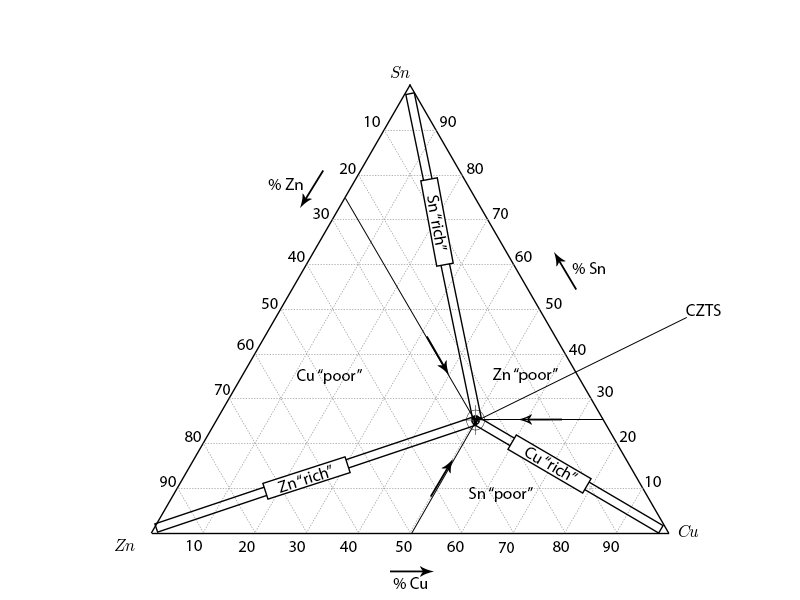
\includegraphics[width=80mm]{ZnSSn2S3Cu2S-general}
    \caption{Location of CZTS, and labelled secondary phases.}
    \label{fig:ZnSSn2S3Cu2S}
\end{figure}


%------------------------------------------------
\clearpage
\appendix
% Table generated by Excel2LaTeX from sheet '298K'
\begin{table}[htbp]
\chapter{Appendix 1}
  \centering
  \begin{adjustbox}{width=1\textwidth}
    \begin{tabular}{rrrrrrrrrrrrrrrrr}
    \toprule
    \multicolumn{17}{c}{Phase Diagram Data} \\
    \midrule
    Phase & Name  & state & Gibbs Free Energy/kJ mol-1 & Ref   & Enthalpy H/kJ mol-1 & Err   & Ref   & Entropy/J K-1mol-1 & Err   & Ref   & Gibbs Energy of formation /kJ mol-1 & Err   & Ref   & Melting Point/C & Ref   &  \\
    Cu    & Copper & s     & -9.87 & 155   & 0     &       & 156   & 33.2  &       & 156   & 0     &       & 156   & 1084.62 &       &  \\
    Cu\_1.12S & Yarrowite & s     &       &       &       &       &       &       &       &       & -56.9 & 0.4   & 157   &       &       &  \\
    Cu\_1.39S & Spionkopite & s     &       &       &       &       &       &       &       &       & -64.3 & 0.4   & 157   &       &       &  \\
    Cu\_1.6S & geerite & s     &       &       &       &       &       &       &       &       &       &       & F     & G     &       &  \\
    Cu\_1.75S & anilite & s     &       &       &       &       &       & 98.3  &       & 158   & -76.4 &       & 158   &       &       &  \\
    Cu\_1.78S & roxbyite & s     &       &       &       &       &       &       &       &       &       &       & H     & G     &       &  \\
    Cu\_1.85S &       & s     &       &       &       &       &       &       &       &       &       &       &       & J     &       &  \\
    Cu\_1.85S & digenite & s     &       &       &       &       &       &       &       &       & -78.7 & G     & 160   &       &       &  \\
    Cu\_1.934S & djurleite & s     &       &       & -79.75 & 0.4   & 157   & 110   & 4     & 157   & -83.9 & 0.4   & 157   &       &       &  \\
    Cu\_1.965S & djurleite & s     &       &       & -80.25 & 0.4   & 157   & 111   &       & 157   & -84.6 & 0.4   & 157   &       &       &  \\
    Cu\_1.9S &       & n/a   &       &       &       &       &       &       &       &       &       &       &       & K     &       &  \\
    Cu\_2 &       & g     &       &       & 484.17 &       & 161   & 241.5 &       & 161   & 431.96 &       & 161   &       &       &  \\
    Cu\_2S & chalcocite & s     &       &       & -79.5 &       &       & 120.9 &       & 156   & -86.2 &       & 156   & 1100  &       &  \\
    Cu\_3Sn &       & s     &       &       & -31.8 &       & 162   &       &       &       & -11.318 & L     & 163   &       &       &  \\
    CuS   & covellite & s     &       &       & -53.1 &       & 156   & 66.5  &       & 156   & -53.6 &       & 156   & 507M  &       &  \\
    CuS\_2 & vallamininite & n/a   &       &       &       &       &       &       &       &       &       &       &       & J     &       &  \\
    CuSn  &       & g     &       &       &       &       &       &       &       &       &       &       &       & J     &       &  \\
    S     &       & cr,mono &       &       &       &       &       &       &       &       &       &       &       & J     &       &  \\
    S     &       & cr,rhombic & -9.506 & 155   & 0     &       & 156   & 32.1  &       & 156   & 0     &       & 156   & 119   &       &  \\
    S     &       & g     & 229.39 & 155   & 277.2 &       & 156   & 167.8 &       & 156   & 236.7 &       & 156   & 115.21 &       &  \\
    S\_2  &       & g     & 60.67 & 155   & 128.6 &       & 156   & 228.2 &       & 156   & 79.7  &       & 156   &       &       &  \\
    S\_3  &       & g     & 64.165 & 155   & 132.6 &       & 162   &       &       &       & 92.68 &       & P     &       &       &  \\
    S\_4  &       & g     & 91.1  & 155   & 136.8 &       & 162   &       &       &       & 119.6 &       & P     &       &       &  \\
    S\_5  &       & g     & 15.32 & 155   & 123.8 &       & 162   &       &       &       & 43.84 &       & P     &       &       &  \\
    S\_6  &       & g     & -6.769 & 155   & 102.5 &       & 162   &       &       &       & 21.75 &       & P     &       &       &  \\
    S\_7  &       & g     & -14.57 & 155   & 113.4 &       & 162   &       &       &       & 13.95 &       & P     &       &       &  \\
    S\_8  &       & g     & -29.317 & 155   & 101.277 &       & 156   & 432.536 &       & 156   & -0.7991 &       & 156   & 95M   &       &  \\
    Sn    &       & cr, white & -15.26 & 155   & 0     &       & 156   & 51.2  &       & 156   & 0     &       & 156   & 231.93 &       &  \\
    Sn    &       & cr, gray &       &       & -2.1  &       & 156   & 44.1  &       & 156   & 0.1   &       & 156   & 13.2M &       &  \\
    Sn\_2S\_3 &       & s     & -312.6 & 155   &       &       &       & 163.6 & 6     & 166   & -235.6 &       & P     & 760   &       &  \\
    Sn\_3S\_4 &       & s     & 442.88 & 155   &       &       &       &       &       &       & 526.7 &       & P     &       &       &  \\
    SnS   &       & g     & 0.032869 & 155   & 119.2 &       & 162   & 242.3 &       & 168   &       &       &       &       &       &  \\
    SnS   &       & s     &       &       & -100  &       & 156 162 & 77    &       & 156   & -98.3 &       & 156   & 880   &       &  \\
    SnS\_2 &       & s     & -179.62 & 155   & -15.55 &       & 169   & 87.5  &       & 169   & -145.394 &       & 169   & 745   &       &  \\
    Zn    &       & s     & -12.41 & 155   & 0     &       & 156   & 41.6  &       & 156   & 0     &       & 156   & 419.53 &       &  \\
    Zn    &       & g     &       &       & 130.4 &       & 156   & 160.1 &       & 156   & 94.8  &       & 156   &       &       &  \\
    ZnS   & sphaelerite & cr    & -222.375 & 155   & -206  &       & 156   & 57.7  &       & 156   & -201.3 &       & 156   & 1700  &       &  \\
    ZnS   & Wurzite & cr    & -212.107 & 155   & -192.6 &       & 156   &       &       &       & -190.2 &       & P     & 1700  &       &  \\
    ZnS   &       & g     & 128.239 & 155   &       &       &       &       &       &       & 137.75 &       & P     &       &       &  \\
    ZnSn  &       &       &       &       &       &       &       &       &       &       &       &       &       & K     &       &  \\
    a-Cu0.61Zn0.39 &       & s     &       &       & -9.37 &       & 164   & 2.8   &       & 164   & 0.67  &       & P     &       &       &  \\
    a-Cu0.65Zn0.35 &       & s     &       &       & -8.891 &       & 164   & 2.89  &       & 164   & 1     &       & P     &       &       &  \\
    a-Cu0.70Zn0.3 &       & s     &       &       & -7.97 &       & 164   & 2.89  &       & 164   & 1.8   &       & P     &       &       &  \\
    a-Cu0.75Zn0.25 &       & s     &       &       & -7.03 &       & 164   & 2.89  &       & 164   & 2.6   &       & P     &       &       &  \\
    a-Cu0.80Zn0.20 &       & s     &       &       & -5.86 &       & 164   & 2.72  &       & 164   & 3.7   &       & P     &       &       &  \\
    a-Cu0.85Zn0.15 &       & s     &       &       & -4.52 &       & 164   & 2.43  &       & 164   & 5     &       & P     &       &       &  \\
    a-Cu0.90Zn0.10 &       & s     &       &       & -3.09 &       & 164   & 2.01  &       & 164   & 6.5   &       & P     &       &       &  \\
    a-Cu0.95Zn0.05 &       & s     &       &       & -1.58 &       & 164   & 1.3   &       & 164   & 8     &       & P     &       &       &  \\
    b-Cu0.45Zn0.55 &       & s     &       &       & -9.455 &       & 164   & 3.72  &       & 164   &       &       &       & J     &       &  \\
    b'-Cu0.5Zn0.5 &       & s     &       &       & -11.296 &       & 164   & 1.2552 &       & 164   & -0.52 &       & P     &       &       &  \\
    b-Cu0.5Zn0.5 &       & s     &       &       & -9.142 &       & 164   & 4.18  &       & 164   &       &       &       & J     &       &  \\
    b-Cu0.52Zn0.48 &       & s     &       &       & -11.338 &       & 164   & 0.92  &       & 164   & -0.51 &       & P     &       &       &  \\
    b'-Cu0.55Zn0.45 &       & s     &       &       & -10.37 &       & 164   & 1.97  &       & 164   & 0.063 &       & P     &       &       &  \\
    b-Cu0.55Zn0.45 &       & s     &       &       & -8.49 &       & 164   & 4.56  &       & 164   &       &       &       & J     &       &  \\
    b-Cu0.60Zn0.40 &       & s     &       &       & -7.69 &       & 164   & 4.85  &       & 164   &       &       &       & J     &       &  \\
    b-Cu0.615Zn0.385 &       & s     &       &       & -7.44752 &       & 164   & 4.89  &       & 164   &       &       &       & J     &       &  \\
    g-Cu0.32Zn0.68 &       & s     &       &       & -10.66 &       & 164   & 1.13  &       & 164   & 0.6   &       & P     &       &       &  \\
    g-Cu0.385Zn0.615 &       & s     &       &       & -12.34 &       & 164   & 0.54  &       & 164   & -1.05 &       & P     &       &       &  \\
    g-Cu0.415Zn0.585 &       & s     &       &       & -11.715 &       & 164   & 1.46  &       & 164   & -0.776 &       & P     &       &       &  \\
    d-Cu0.265Zn0.735 &       & s     &       &       & n/a   &       & 164   & n/a   &       & 164   &       &       &       & J     &       &  \\
    e-Cu0.15Zn0.85 &       & s     &       &       & -5.355 &       & 164   & 1     &       & 164   & 6.4   &       & P     &       &       &  \\
    e-Cu0.18Zn0.82 &       & s     &       &       & n/a   &       & 164   & n/a   &       & 164   & n/a   &       & P     &       &       &  \\
    e-Cu0.21Zn0.79 &       & s     &       &       & -7.196 &       & 164   & 0.836 &       & 164   & 4.4   &       & P     &       &       &  \\
    n'-Cu6Sn5 &       & s     & -43.22 & 170   &       &       &       &       &       &       & -30.9 & L     & 170   &       &       &  \\
    n-Cu6Sn5 &       & s     & -43.96 & 170   &       &       &       &       &       &       &       &       &       & J     &       &  \\
    Cu2SnS3 &       & cr    &       &       & -227.8 &       & 52    &       &       &       &       &       &       & 847   &       &  \\
    Cu2ZnSnS4 &       & cr    &       &       & -406  &       & 52    &       &       &       &       &       &       &       &       &  \\
          &       &       &       &       &       &       &       &       &       &       &       &       &       &       &       &  \\
    \bottomrule
    \end{tabular}%
    \end{adjustbox}
  \label{tab:addlabel}%
\end{table}%


\clearpage

\begin{figure}[t]
\chapter{Appendix 2}
\centering
\begin{subfigure}{70mm}
  \centering
    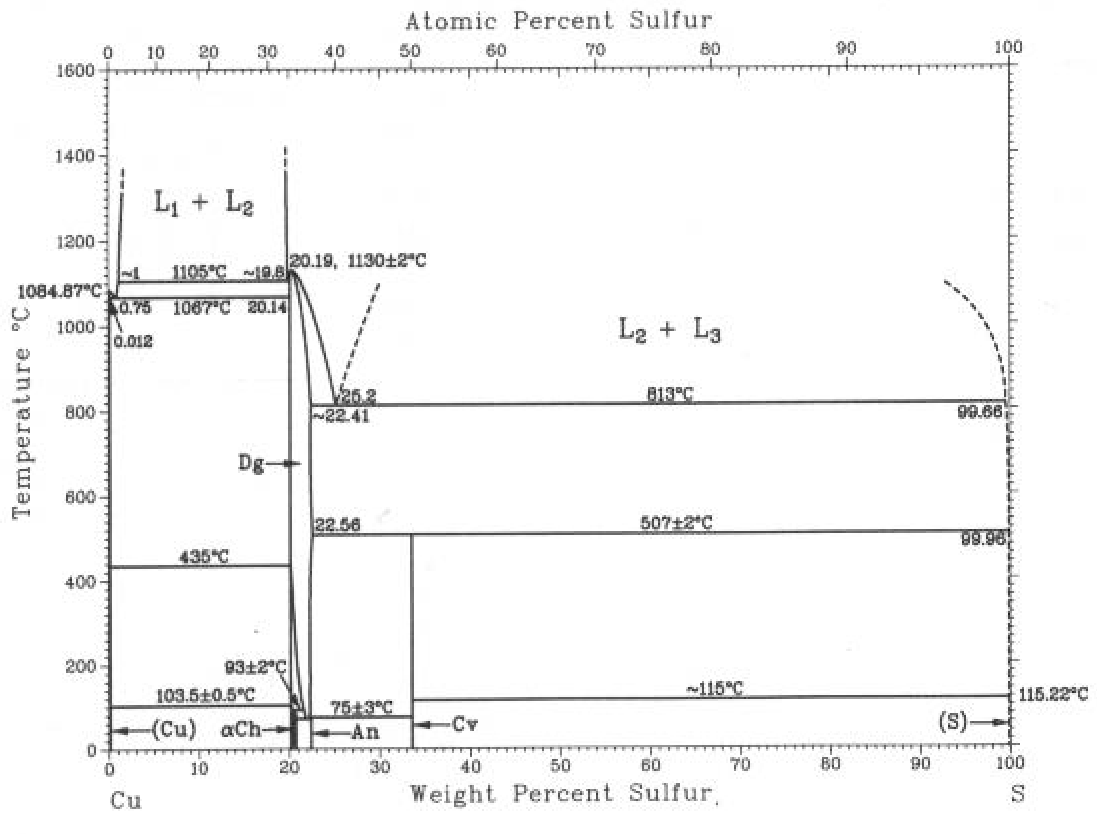
\includegraphics[width=70mm]{CuSAlloyDiag.png}
    \caption{Cu, S Binary Phase Diagram\citep{Hay2000}}
    \label{fig:CuS}
\end{subfigure}%
\begin{subfigure}{70mm}
 \centering
    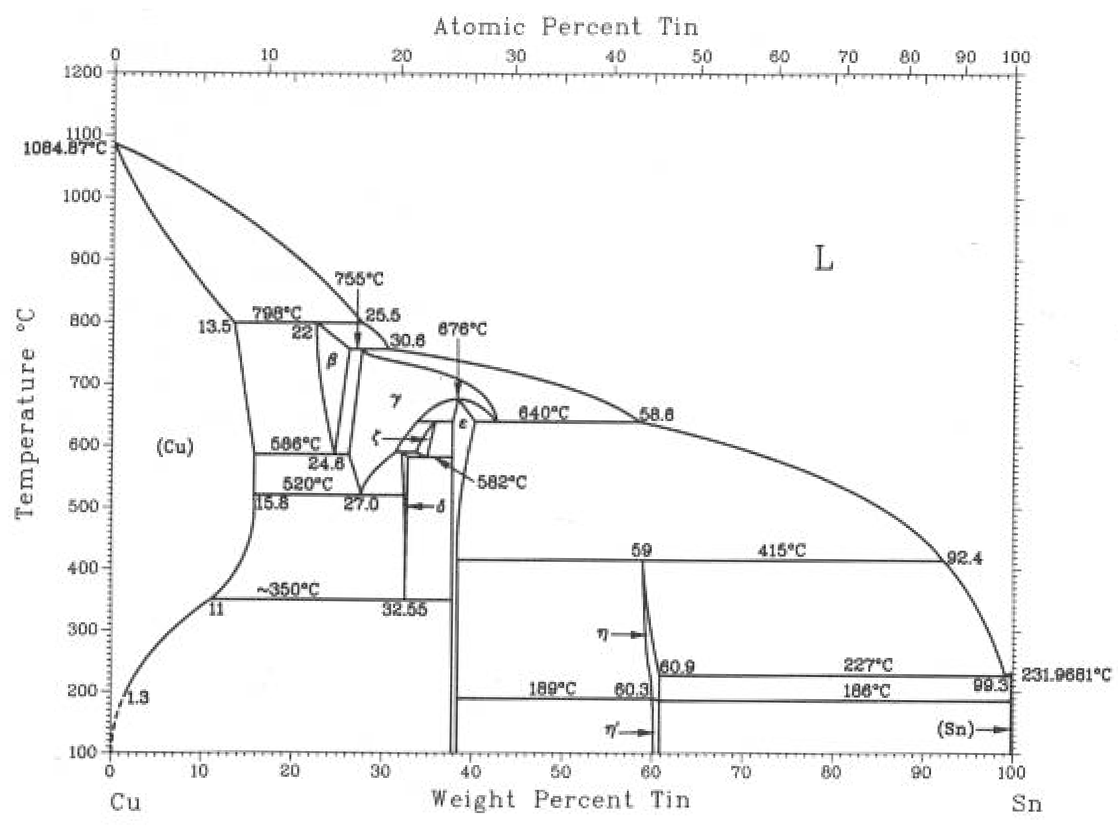
\includegraphics[width=70mm]{CuSnAlloyDiag.png}
    \caption{Cu, Sn Binary Phase Diagram\citep{Hay2000}}
    \label{fig:CuSn}
\end{subfigure}
\begin{subfigure}{70mm}
 \centering
    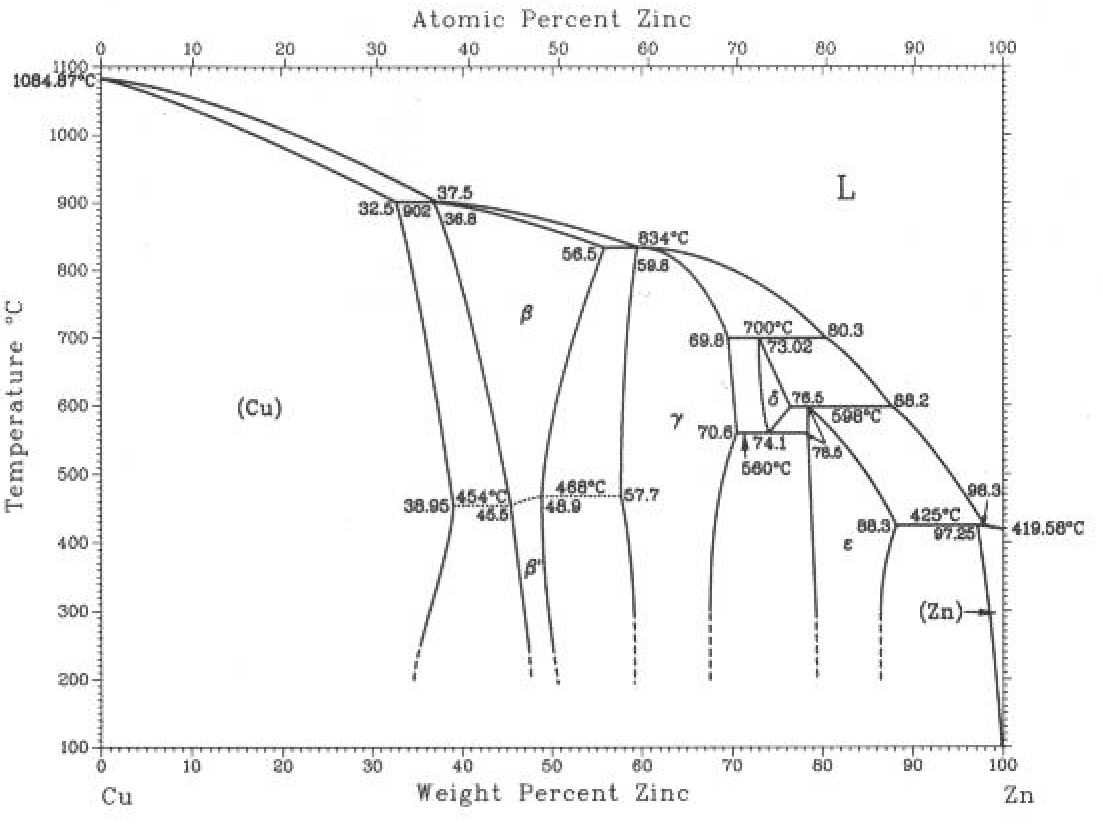
\includegraphics[width=70mm]{CuZnAlloyDiag.png}
    \caption{Cu, Zn Binary Phase Diagram\citep{Hay2000}}
    \label{fig:CuZn}
\end{subfigure}
\begin{subfigure}{70mm}
 \centering
    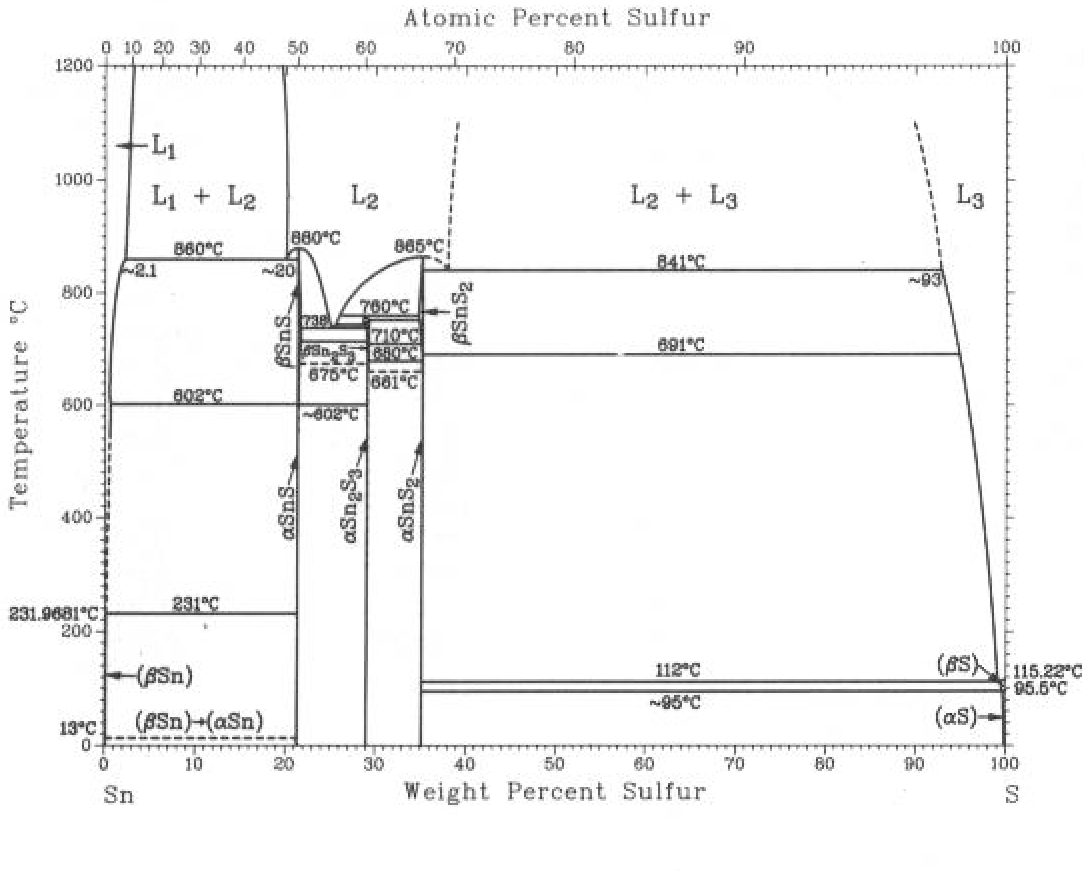
\includegraphics[width=70mm]{SnSAlloyDiag.png}
    \caption{Sn, S Binary Phase Diagram\citep{Hay2000}}
    \label{fig:SnS}
\end{subfigure}
\begin{subfigure}{70mm}
 \centering
    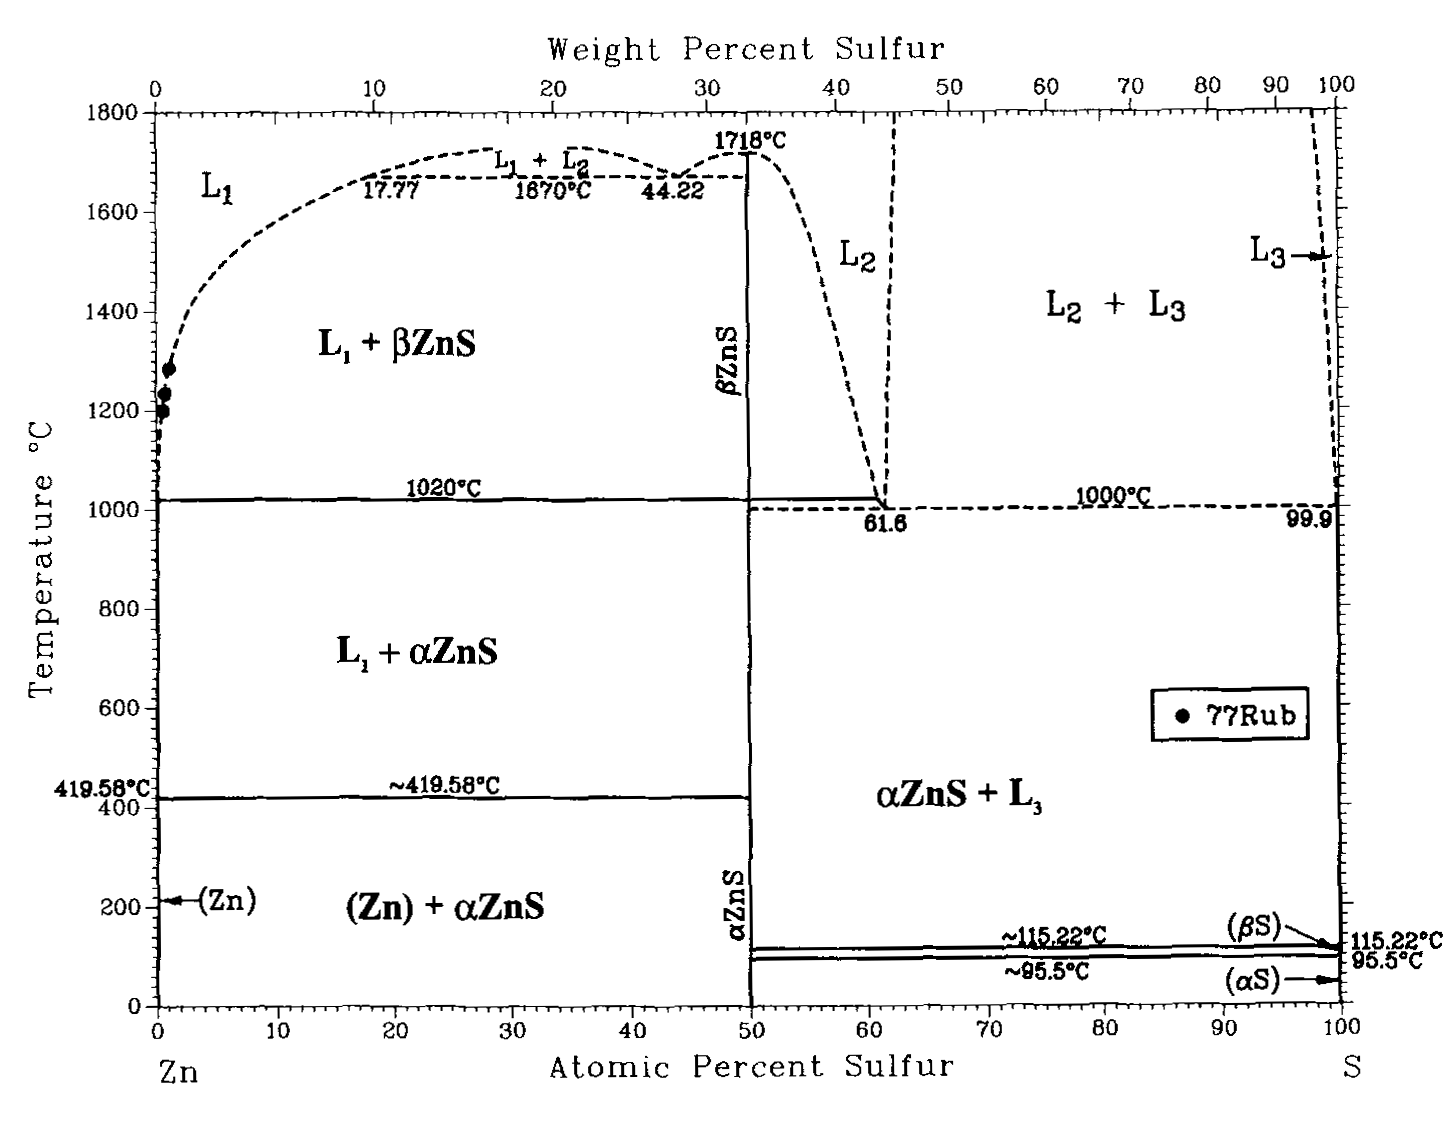
\includegraphics[width=70mm]{ZnSAlloyDiag.png}
    \caption{Zn, S Binary Phase Diagram\citep{Sharma1996}}
    \label{fig:ZnS}
\end{subfigure}
\begin{subfigure}{70mm}
 \centering
    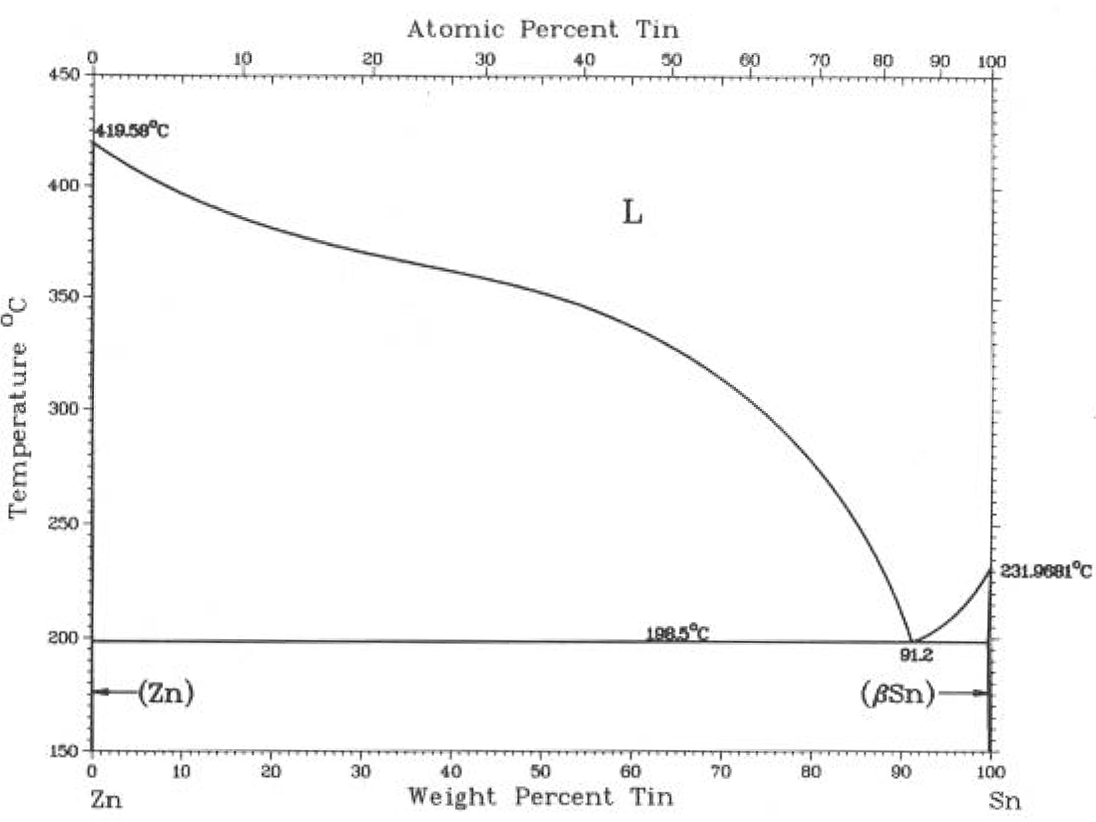
\includegraphics[width=70mm]{ZnSnAlloyDiag.png}
    \caption{Zn, Sn Binary Phase Diagram\citep{Hay2000}}
    \label{fig:ZnSn}
\end{subfigure}
\caption{Binary Alloy Phase Diagrams Used in the calculation of the Ternary Phase Diagrams.}
\label{fig:BinaryAlloyPhaseDiagrams}
\end{figure}

%----------------------------------------------------------------------------------------
%	REFERENCE LIST
%----------------------------------------------------------------------------------------
\clearpage
\bibliography{zotero}
\bibliographystyle{plainnat}


%----------------------------------------------------------------------------------------

%\end{multicols}

\end{document}
